\documentclass[11pt,a4paper]{article}
\usepackage[utf8]{inputenc}
\usepackage[T1]{fontenc}
\usepackage{lmodern}
\usepackage[margin=2.5cm]{geometry}
\usepackage{enumitem}
\usepackage{booktabs}
\usepackage{multirow}
\usepackage{hyperref}
\usepackage{xcolor}
\usepackage{amsmath,amssymb}
\usepackage{caption}
\usepackage{float}
\usepackage{graphicx}
\usepackage{natbib}

% Resolve image paths from repo root (needed for Overleaf)
\graphicspath{{../}}

\hypersetup{colorlinks=true, linkcolor=blue!70!black, urlcolor=blue!60!black, citecolor=green!50!black}

\title{\textbf{Cross-Fitting Under Dependent Data:}\\[4pt]
\large Replication \& Extension of Balkus, Laith \& Hejazi (2026)}
\author{[Author Name]\\Master Thesis --- [University]}
\date{June 2026}

\begin{document}
\maketitle

%======================================================================
\section{Background}
%======================================================================

When we use machine learning to estimate causal effects, the ML model can overfit: it learns patterns that don't generalize. This creates \emph{empirical process (EP) bias} --- a systematic error caused by using the same data for nuisance estimation and inference. \emph{Cross-fitting} fixes this by splitting the data: train the ML model on one half, estimate the causal effect on the other, then swap \citep{chernozhukov2018}. A learner that doesn't overfit enough to create EP bias is called ``Donsker-class'' --- for such learners, cross-fitting is unnecessary \citep[p.~C16]{chernozhukov2018}.

But what if units are correlated --- e.g., students in schools, or workers in firms? \citet{chiang2021} argue that splits must \emph{respect} the clustering: correlated units cannot be in different folds. They propose K$^2$-fold splitting, which partitions both row and column clusters into $K$ groups. The downside: with $K=2$, each training fold sees only $\sim$25\% of the data.

\citet{balkus2026} prove this elaborate splitting is \textbf{usually unnecessary}. Their Theorem~1 shows that plain random splitting --- ignoring clusters --- still eliminates EP bias, as long as cluster sizes don't grow with the sample. They call this ``as-IID'' splitting. One caveat: even though the \emph{splitting strategy} doesn't need to know about clusters, the \emph{standard errors} still do:
\begin{quote}
\emph{``Variance estimates used for the construction of confidence intervals must be adjusted to account for inter-unit correlation.''} --- \citet[Section~4]{balkus2026}
\end{quote}

This distinction --- splitting strategy vs.\ standard error formula --- is the central theme of this report.

\paragraph{Three strategies we compare.}
\begin{itemize}[leftmargin=1.5em, nosep]
  \item \textbf{No CF}: No splitting. Train and predict on the same data.
  \item \textbf{As-IID}: Standard random $K$-fold splitting, ignoring clusters.
  \item \textbf{Chiang K$^2$-fold}: Cluster-aware splitting that guarantees independence between training and test data.
\end{itemize}

\paragraph{Standard errors.} Chiang et al.\ use the classical two-way cluster-robust variance $\hat{V} = V_{\text{row}} + V_{\text{col}} - V_{\text{iid}}$ from \citet{cameron2011}, applied to DML influence function scores. We use this same formula across all three strategies, so any coverage difference is due to the splitting strategy alone.

\paragraph{Why not DoubleML?} The \texttt{DoubleML} library bundles splitting and SE estimation into a single toggle: setting \texttt{cluster\_cols} gives K$^2$-fold splitting \emph{and} cluster-robust SEs; leaving it unset gives as-IID splitting \emph{and} IID SEs. The combination Balkus recommends --- as-IID + cluster-robust SEs --- is unavailable. We therefore translated Balkus's R code into Python and added the Cameron et al.\ (2011) formula on top, giving us a $3 \times 2$ factorial design (strategy $\times$ SE type). See Section~\ref{sec:doubleml} for validation.


%======================================================================
\section{How We Measure Success}
\label{sec:morris}
%======================================================================

We run each experiment 200 times with different seeds. Each run produces an estimate $\hat{\theta}$ and a standard error $\widehat{SE}$. Because we control the DGP, we know the true $\theta_0$.

Following \citet{morris2019}, we compute:
\begin{itemize}[leftmargin=1.5em, nosep]
  \item \textbf{Bias}: $\bar{\hat{\theta}} - \theta_0$. Is the estimator centered on the truth?
  \item \textbf{EmpSE}: $\text{SD}(\hat{\theta})$ across replications. The true sampling variability.
  \item \textbf{ModSE}: $\sqrt{\text{mean}(\widehat{SE}^2)}$. What the formula \emph{thinks} the uncertainty is.
  \item \textbf{RelSE = ModSE / EmpSE}: Are the reported SEs correct? Values below 1 mean SEs are too small.
  \item \textbf{Coverage}: How often does the 95\% CI contain $\theta_0$?
\end{itemize}

RelSE is more informative than coverage alone: two methods can both have 88\% coverage, but one might have RelSE $= 0.90$ (slightly fixable) while the other has RelSE $= 0.39$ (fundamentally broken).


%======================================================================
\section{Balkus Replication: Which Learner Needs Cross-Fitting?}
\label{sec:balkus}
%======================================================================

We test three ML learners on Balkus's two-way clustered DGP, each at a different point on the overfitting spectrum:

\begin{itemize}[leftmargin=1.5em, nosep]
  \item \textbf{MARS} (R's \texttt{earth}): Additive splines with built-in GCV pruning. Approximately Donsker.
  \item \textbf{Deep RF} (sklearn): Fully-grown random forests that memorize training data. Not Donsker --- exactly what cross-fitting was invented for.
  \item \textbf{Lasso}: L1-regularized regression. Not technically Donsker, but regularization keeps EP bias small enough that it \emph{behaves} like a careful learner.
\end{itemize}

All results use Balkus's original DGP (a direct replication of their R code in Python).


\subsection{MARS Doesn't Need Cross-Fitting}

\begin{figure}[H]
\centering
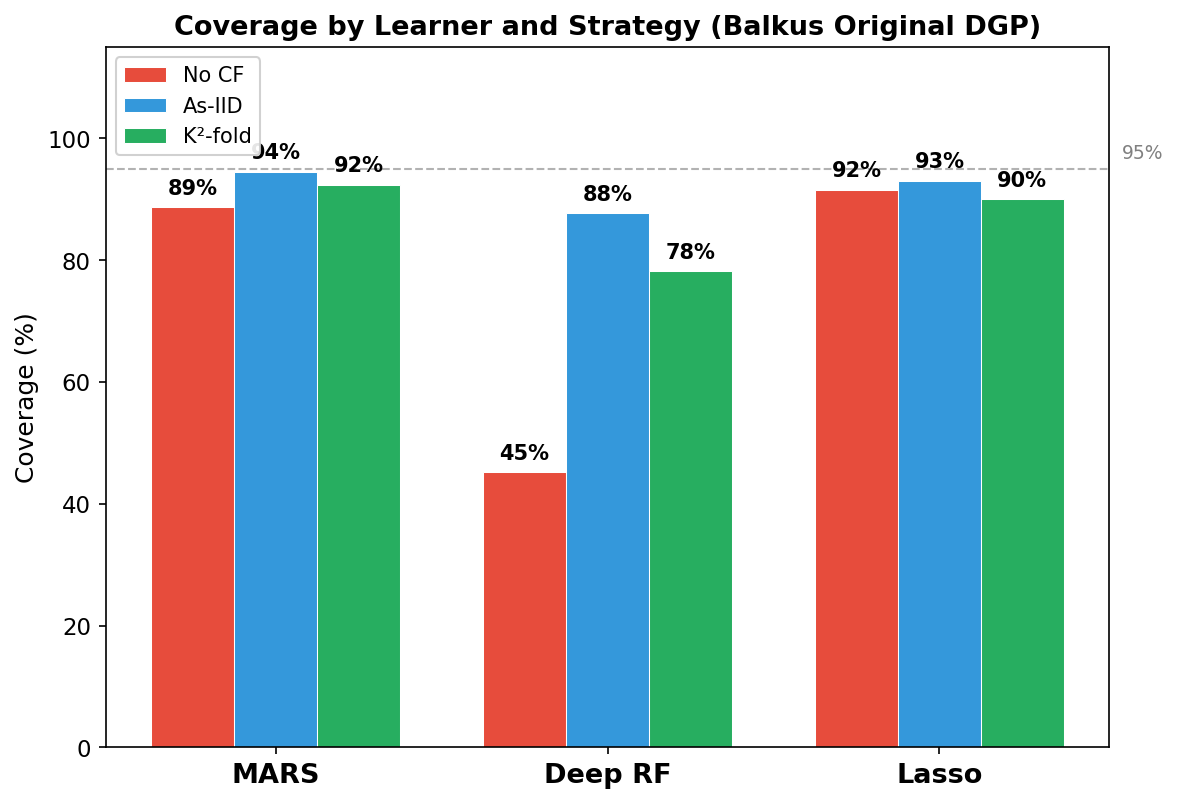
\includegraphics[width=\textwidth]{replications/balkus/results/plots/mars_vs_deep_rf.png}
\caption{Coverage by learner and strategy on the Balkus Original DGP (averaged over three sample sizes).}
\label{fig:mars-vs-rf}
\end{figure}

MARS achieves 89--92\% coverage \emph{without any cross-fitting}. Its GCV pruning prevents the overfitting that creates EP bias. This makes MARS the wrong learner to test Balkus's theorem: if cross-fitting doesn't matter regardless, we can't tell whether as-IID splitting ``works'' or whether splitting is just irrelevant. That's why we introduced Deep RF.

\paragraph{Bias and variance by learner.} On the original DGP at $n=2500$ ($50 \times 50$ grid), the three learners show very different bias profiles without cross-fitting: MARS has near-zero bias (${+}0.005$, EmpSE $= 0.054$), confirming it doesn't overfit. Lasso is similarly well-behaved (bias ${+}0.003$, EmpSE $= 0.053$). Deep RF, by contrast, shows systematic negative bias ($-0.040$, EmpSE $= 0.059$) --- the bias is what kills coverage (RelSE $= 0.40$), not the variance. With as-IID cross-fitting, Deep RF's bias drops to ${+}0.032$ and EmpSE rises to $0.095$ (the model generalizes better but each fold sees less data), recovering coverage to 88\%.

\paragraph{Data starvation under K$^2$-fold.} K$^2$-fold splits also eliminate Deep RF's EP bias, but EmpSE increases further: at $n=2500$, MARS EmpSE goes from $0.054$ (no CF) to $0.462$ (as-IID) to $1.164$ (K$^2$-fold). The K$^2$-fold training sets are only $\sim$25\% of the data, so the nuisance estimates become noisy and the treatment effect estimates inherit that variance.


\subsection{SE Calibration and Decoupling}

Coverage shows whether CIs work; RelSE shows why they fail. Figure~\ref{fig:morris-relse} shows SE calibration under both IID and cluster-robust (CR) SEs.

\begin{figure}[H]
\centering
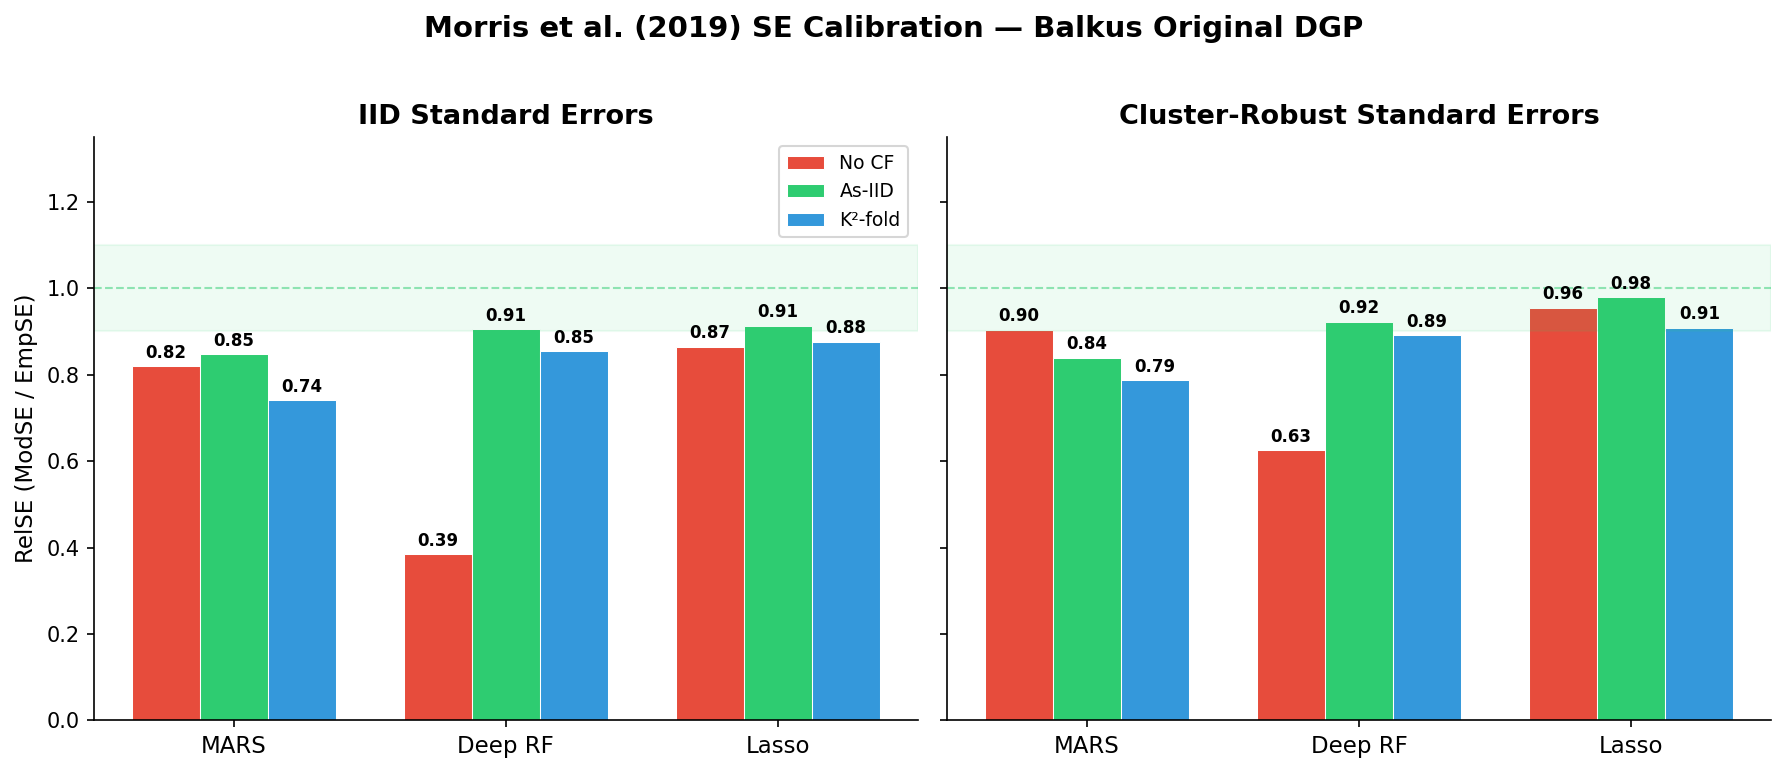
\includegraphics[width=\textwidth]{replications/balkus/results/plots/morris_relse_dual.png}
\caption{Morris et al.\ (2019) SE calibration on the Balkus Original DGP. RelSE close to 1.0 (green zone) means well-calibrated SEs. Left: IID SEs. Right: cluster-robust SEs.}
\label{fig:morris-relse}
\end{figure}

Table~\ref{tab:decoupling} gives the full $3 \times 2$ breakdown. The key patterns:

% Auto-generated from CSV: python -m report.generate_tables
\begin{table}[H]
\centering\small
\caption{Coverage and RelSE by strategy and SE type, Balkus DGP variants (averaged over sample sizes). Bold = closest to 95\%.}
\label{tab:decoupling}
\begin{tabular}{llrrrr}
\toprule
\textbf{Learner} & \textbf{Strategy} & \textbf{Cov.\ (IID SE)} & \textbf{Cov.\ (CR SE)} & \textbf{RelSE (IID)} & \textbf{RelSE (CR)} \\
\midrule
  \multirow{3}{*}{MARS} & no\_cf & 88.7\% & \textbf{90.5\%} & 0.82 & 0.90 \\
   & as\_iid & \textbf{94.5\%} & 93.5\% & 0.85 & 0.84 \\
   & chiang & \textbf{92.3\%} & 91.7\% & 0.74 & 0.79 \\
\midrule
  \multirow{3}{*}{Deep RF} & no\_cf & 45.2\% & \textbf{63.7\%} & 0.39 & 0.63 \\
   & as\_iid & \textbf{87.7\%} & 85.5\% & 0.91 & 0.92 \\
   & chiang & 78.2\% & \textbf{78.7\%} & 0.85 & 0.89 \\
\midrule
  \multirow{3}{*}{LASSO} & no\_cf & 91.5\% & \textbf{92.0\%} & 0.87 & 0.96 \\
   & as\_iid & \textbf{93.0\%} & 92.3\% & 0.91 & 0.98 \\
   & chiang & 90.0\% & \textbf{92.3\%} & 0.87 & 0.94 \\
\bottomrule
\end{tabular}
\end{table}

\begin{itemize}[leftmargin=1.5em, nosep]
  \item \textbf{Deep RF without CF is broken}: RelSE $= 0.39$ with IID SEs. CR SEs improve it to $0.63$ but cannot fix EP bias --- coverage stays below 65\%.
  \item \textbf{Cross-fitting fixes Deep RF}: as-IID brings RelSE to $\sim$0.92 regardless of SE type.
  \item \textbf{MARS and Lasso barely need cross-fitting}: their RelSE is 0.82--0.87 without CF. CR SEs bring MARS to 0.90 even without splitting.
  \item \textbf{Lasso as-IID + CR SE achieves RelSE $= 0.98$} --- nearly perfect calibration, the best in the table.
\end{itemize}

\paragraph{Bottom line.} Cross-fitting eliminates EP bias (Chernozhukov's contribution). CR SEs account for remaining cluster correlation. For careful learners, CR SEs alone nearly suffice. For reckless learners, you need \emph{both}.


%======================================================================
\section{Chiang Replication: Testing on Chiang's Own DGP}
\label{sec:chiang}
%======================================================================

We replicate the partially linear IV (PLIV) model from \citet[Section~4.1]{chiang2021} with Lasso and $p = 100$ covariates. Since Lasso's EP bias is small, this tests data starvation and decoupling rather than bias removal.


\subsection{Main Results}

Table~\ref{tab:chiang-decoupling} shows coverage under both IID and CR standard errors for each strategy.

% Auto-generated from CSV: python -m report.generate_tables
\begin{table}[H]
\centering\small
\caption{Chiang PLIV: coverage by SE type, 220 replications. Bold = closer to 95\%. As-IID + CR SE wins in every scenario.}
\label{tab:chiang-decoupling}
\begin{tabular}{llrrrr}
\toprule
\textbf{Scenario} & \textbf{Strategy} & \textbf{Cov.\ (IID SE)} & \textbf{Cov.\ (CR SE)} & \textbf{RelSE (IID)} & \textbf{RelSE (CR)} \\
\midrule
  $(25,25)$, $p=100$ & no\_cf & 80.0\% & \textbf{88.2\%} & 0.67 & 0.85 \\
   & as\_iid & 85.9\% & \textbf{92.7\%} & 0.78 & 0.94 \\
   & chiang\_k2 & 66.8\% & \textbf{87.3\%} & 0.54 & 0.80 \\
\midrule
  $(50,50)$, $p=100$ & no\_cf & 71.4\% & \textbf{91.4\%} & 0.55 & 0.91 \\
   & as\_iid & 74.5\% & \textbf{92.3\%} & 0.61 & 0.93 \\
   & chiang\_k2 & 60.0\% & \textbf{90.9\%} & 0.45 & 0.84 \\
\bottomrule
\end{tabular}
\end{table}

\begin{itemize}[leftmargin=1.5em, nosep]
  \item \textbf{CR SEs improve coverage by 7--20 pp} over IID SEs. Within-cluster correlation is real.
  \item \textbf{As-IID + CR SE wins}: 92.7\% at $(25,25)$, 92.3\% at $(50,50)$.
  \item \textbf{K$^2$-fold suffers from data starvation}: with $K=2$ on a $25 \times 25$ grid, each fold trains on $\sim$144 observations for 100 covariates.
\end{itemize}

Figure~\ref{fig:chiang-se-dual} makes this visual. Each dot is one replication's model SE; the dashed line is the true EmpSE. Well-calibrated SEs cluster on the dashed line.

\begin{figure}[H]
\centering
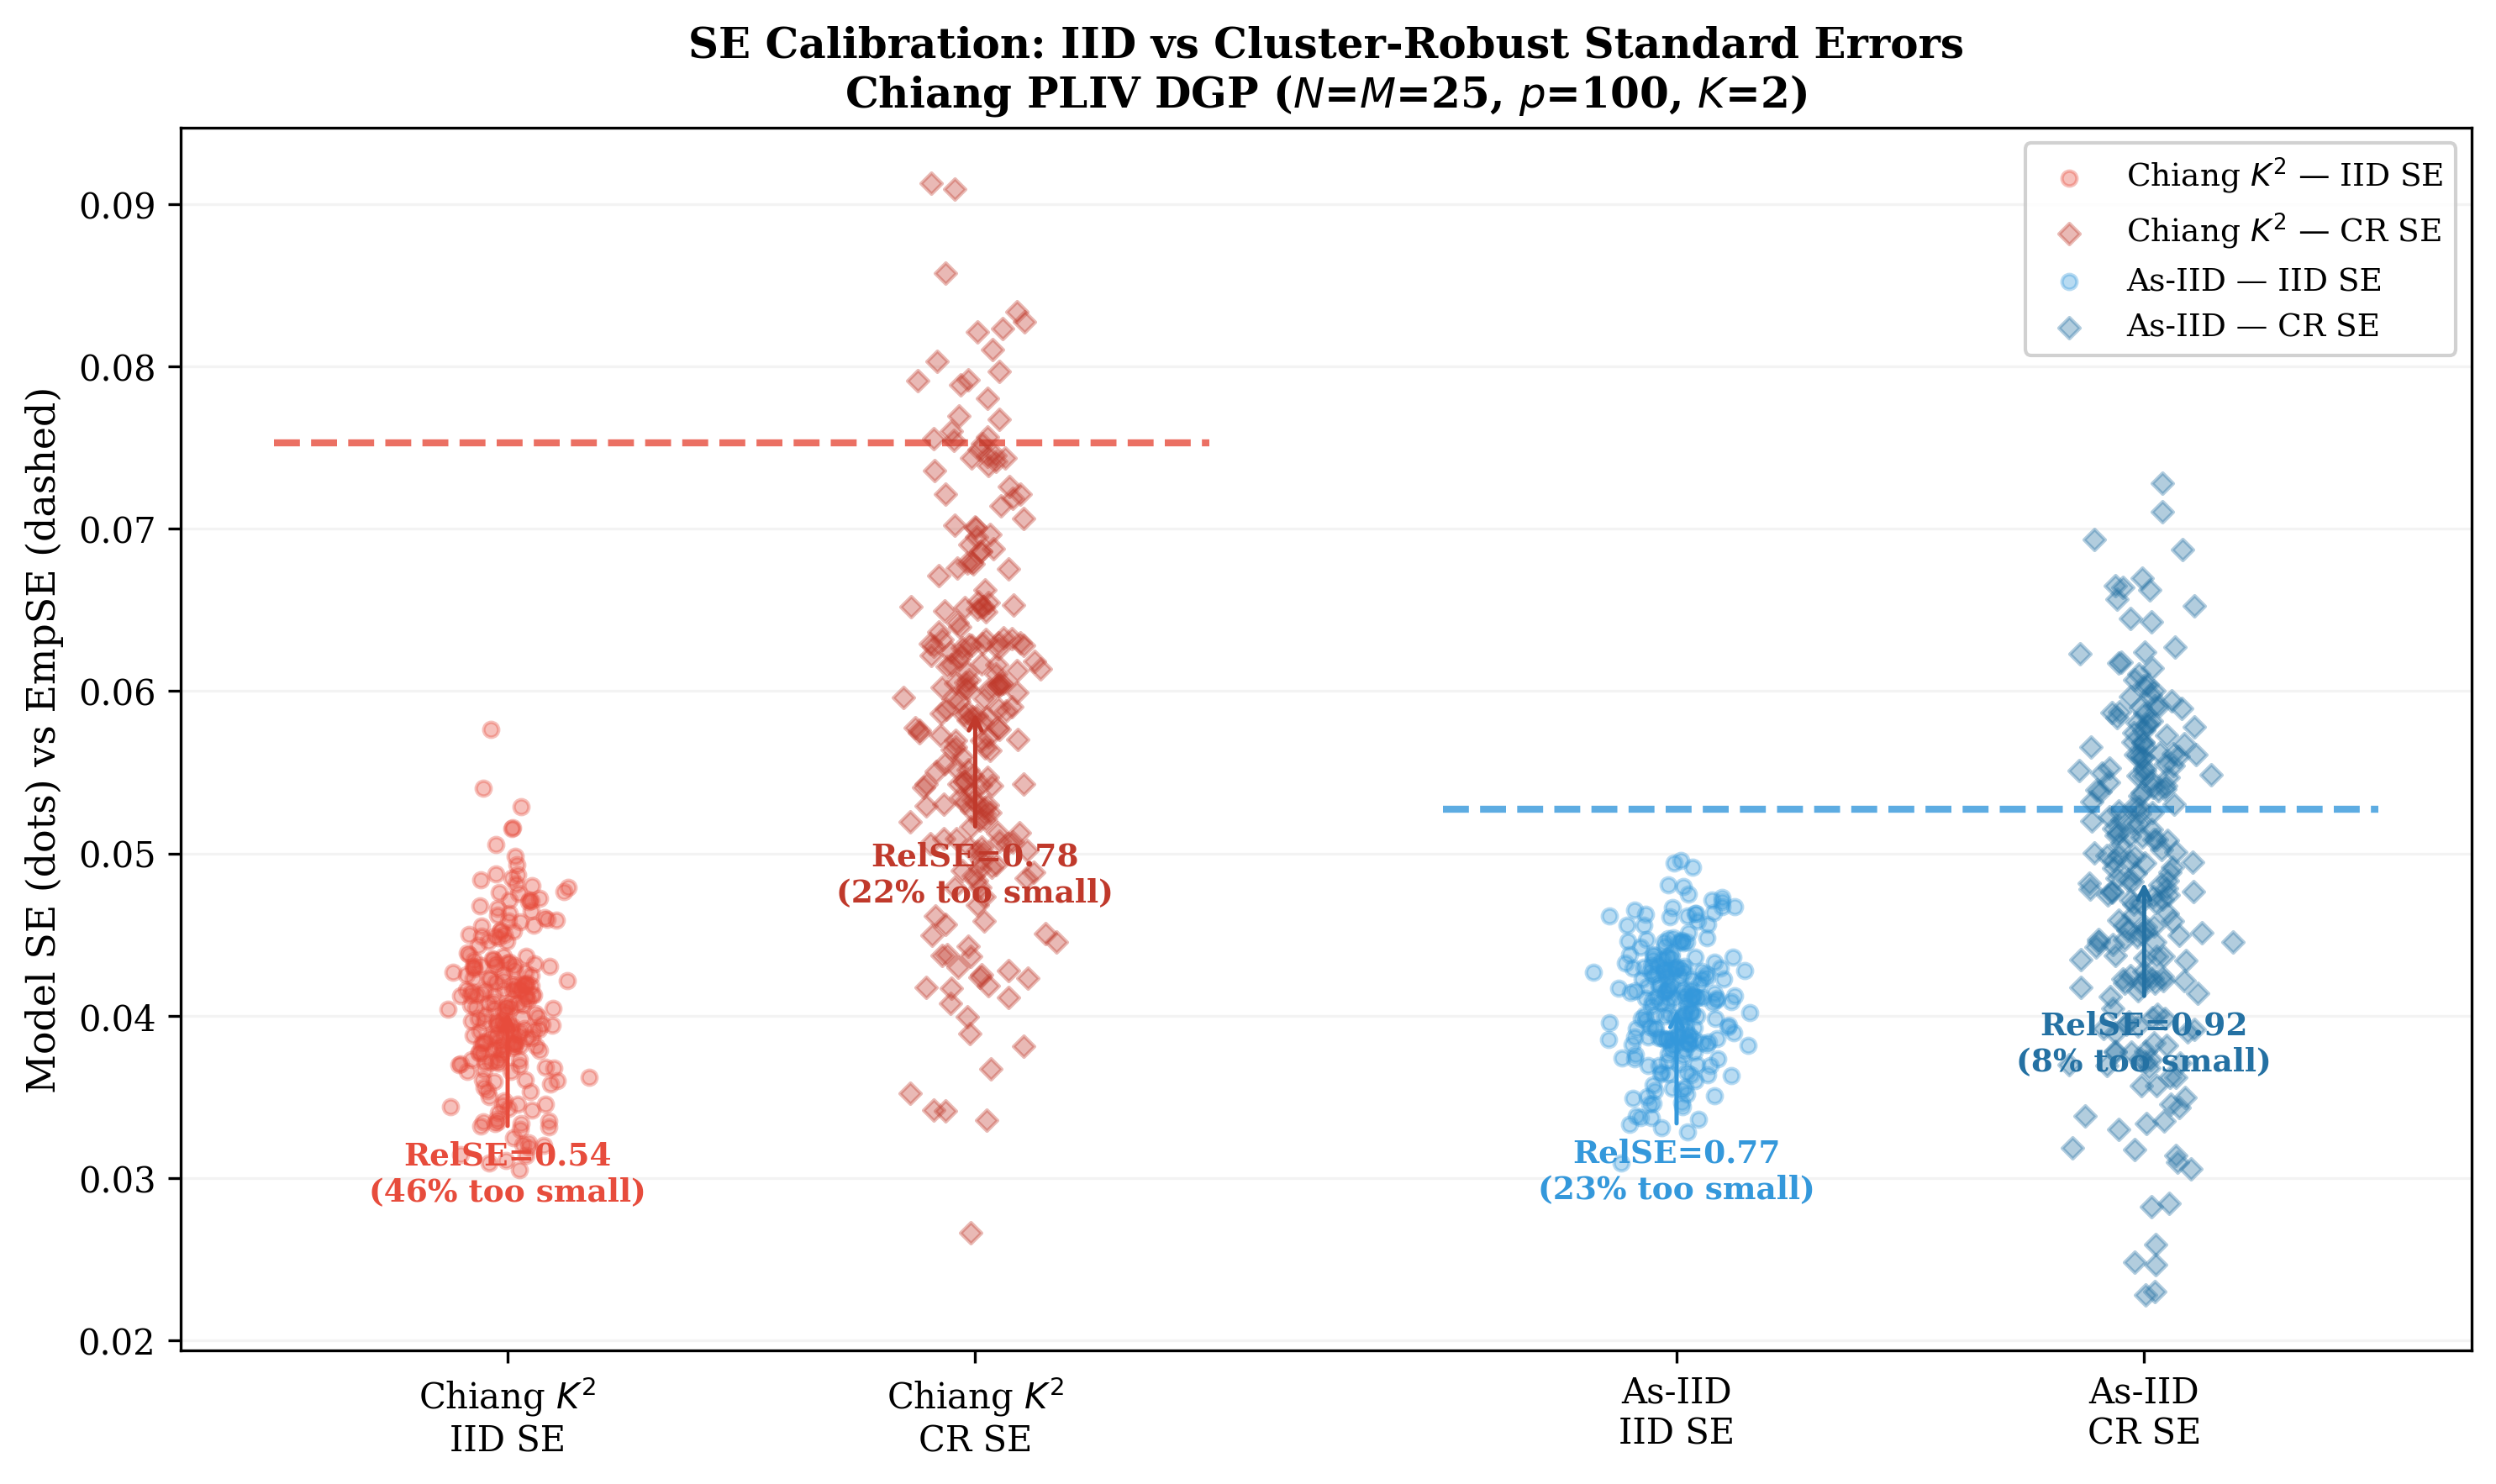
\includegraphics[width=\textwidth]{replications/chiang/results/plots/chiang_se_calibration_dual.png}
\caption{SE calibration on Chiang's DGP ($N$=$M$=25, $p$=100). \textbf{As-IID + CR SE} (rightmost): dots cluster on the dashed line (RelSE $= 0.92$). Chiang $K^2$ + IID SE (leftmost): 46\% too small.}
\label{fig:chiang-se-dual}
\end{figure}

\paragraph{The remaining 8\% gap.} Our CR SEs use the CGM (2011) formula, which is slightly downward-biased with moderate cluster counts ($G = 25$). Bias-corrected estimators (CR2, Bell \& McCaffrey, 2002) would likely close this gap.


\subsection{Robustness Check: The DoubleML Library}
\label{sec:doubleml}

To rule out bugs, we repeated the comparison using the \textbf{official DoubleML library} (v0.11.1) with its built-in DGP. Parameters: $N\!=\!M\!=\!25$, $p\!=\!100$, $K\!=\!2$, LassoCV, 200 replications.

\begin{table}[H]
\centering\small
\caption{Rows 1--2: what DoubleML gives you. Rows 3--4: our implementation, which decouples splitting from SE. Bold = best.}
\label{tab:doubleml}
\begin{tabular}{llrrrrrr}
\toprule
\textbf{Splitting} & \textbf{SE type} & \textbf{Bias} & \textbf{EmpSE} & \textbf{ModSE} & \textbf{RelSE} & \textbf{RMSE} & \textbf{Cov.} \\
\midrule
\multicolumn{8}{l}{\textit{DoubleML library (bundled)}} \\
K$^2$-fold & CR (built-in) & $+$0.016 & 0.076 & 0.093 & 1.23 & 0.077 & 99.5\% \\
As-IID     & IID (forced)  & $+$0.003 & 0.057 & 0.040 & 0.71 & 0.057 &  82.0\% \\
\midrule
\multicolumn{8}{l}{\textit{Our implementation (decoupled)}} \\
K$^2$-fold & CR0 & $+$0.015 & 0.075 & 0.060 & 0.80 & 0.077 & 87.3\% \\
As-IID     & CR0 & $+$0.002 & 0.053 & 0.050 & \textbf{0.94} & \textbf{0.053} & \textbf{92.7\%} \\
\bottomrule
\end{tabular}
\end{table}

DoubleML's two options both miss: Chiang over-covers (SEs 23\% too large), as-IID under-covers (IID SEs ignore clusters). When we decouple splitting from SE, \textbf{as-IID + CR SE wins} with the best RelSE (0.94) and coverage (92.7\%).

The problem is software design. DoubleML bundles two independent choices into one toggle:

\begin{center}\small
\begin{tabular}{lcc}
\toprule
\texttt{cluster\_cols} & \textbf{Splitting} & \textbf{Standard errors} \\
\midrule
Set     & K$^2$-fold (cluster-aware) & Cluster-robust \\
Not set & As-IID (random)            & IID \\
\midrule
\textbf{Not available} & \textbf{As-IID (random)} & \textbf{Cluster-robust} \\
\bottomrule
\end{tabular}
\end{center}

Balkus's theorem tells us these are \emph{logically independent} choices. The optimal combination is the one DoubleML doesn't offer.


%======================================================================
\section{Where the Theory Breaks}
\label{sec:boundary}
%======================================================================

Balkus's Corollary~2 requires that cluster sizes are \emph{bounded} --- each row contains at most $C$ columns, where $C$ doesn't grow with the sample. In a full $N \times M$ grid, every row contains $M$ observations, so $C = M \to \infty$. We tested this with strong cluster effects. Coverage declines from 85\% to 71\% as the grid grows --- for \emph{both} strategies equally. The culprit is the cluster-robust SE formula itself (which assumes fixed cluster sizes), not the splitting strategy. On bounded-cluster DGPs (sparse bipartite graph, $d=20$), both strategies achieve 97\% coverage, confirming the boundary is exactly where the theory predicts.


%======================================================================
\section{Conclusion}
%======================================================================

\begin{enumerate}[leftmargin=1.5em, nosep]
  \item \textbf{Balkus's theorem holds empirically, and whether you need cross-fitting depends on the learner.} As-IID splitting matches or beats K$^2$-fold across two DGPs, three learners, and multiple sample sizes. MARS and Lasso don't need cross-fitting (they don't overfit); Deep RF is catastrophic without it.
  \item \textbf{The real issue is standard errors, not splitting.} When cluster sizes grow with the sample, coverage drops for both strategies --- the CR SE formula breaks down.
  \item \textbf{Software should separate splitting from variance estimation.} DoubleML bundles them, preventing the optimal combination: as-IID splitting + cluster-robust SEs.
  \item \textbf{Practical advice:} Use as-IID cross-fitting. Always use cluster-robust standard errors. If clusters are large, consider bootstrap alternatives.
\end{enumerate}


%======================================================================
\bibliographystyle{apalike}
\bibliography{references}

\end{document}
